%%%% hw3-reqdoc.team3.tex
%%%% Requirements Documentation for sQuire
%%%% Due on BBLearn before class on Tuesday 2/9/2016

\documentclass[11pt]{report}

\usepackage{graphicx}
%\graphicspath{ {images/} }

\marginparwidth 0.5in 
\oddsidemargin 0.25in 
\evensidemargin 0.25in 
\marginparsep 0.25in
\topmargin 0.0in 
\textwidth 6in \textheight 8.5in

\title{sQuire: A Collaborative Software Development Tool}
\author{jank6275, mora5651, boss2849, bolt1003, gall7417, brec9824, snev7821, mars2681}

\begin{document}

\maketitle

\tableofcontents

\chapter{Introduction}

\section{Program Premise}
    \begin{figure}[h!]
        \caption{Squire will be a web-based collaborative software development environment with a project development center. Squire will allow multiple users to edit files and communicate in real time. First, projects are stubbed out by a user and then other users can join and/or vote to support for their favorite projects. After a certain amount of support, planning, and documentation is reached for a project, the project becomes a fully fleged project and then community development can start. Think ``kickstarter for code'' where people pledge their help with the project and not just money.}
        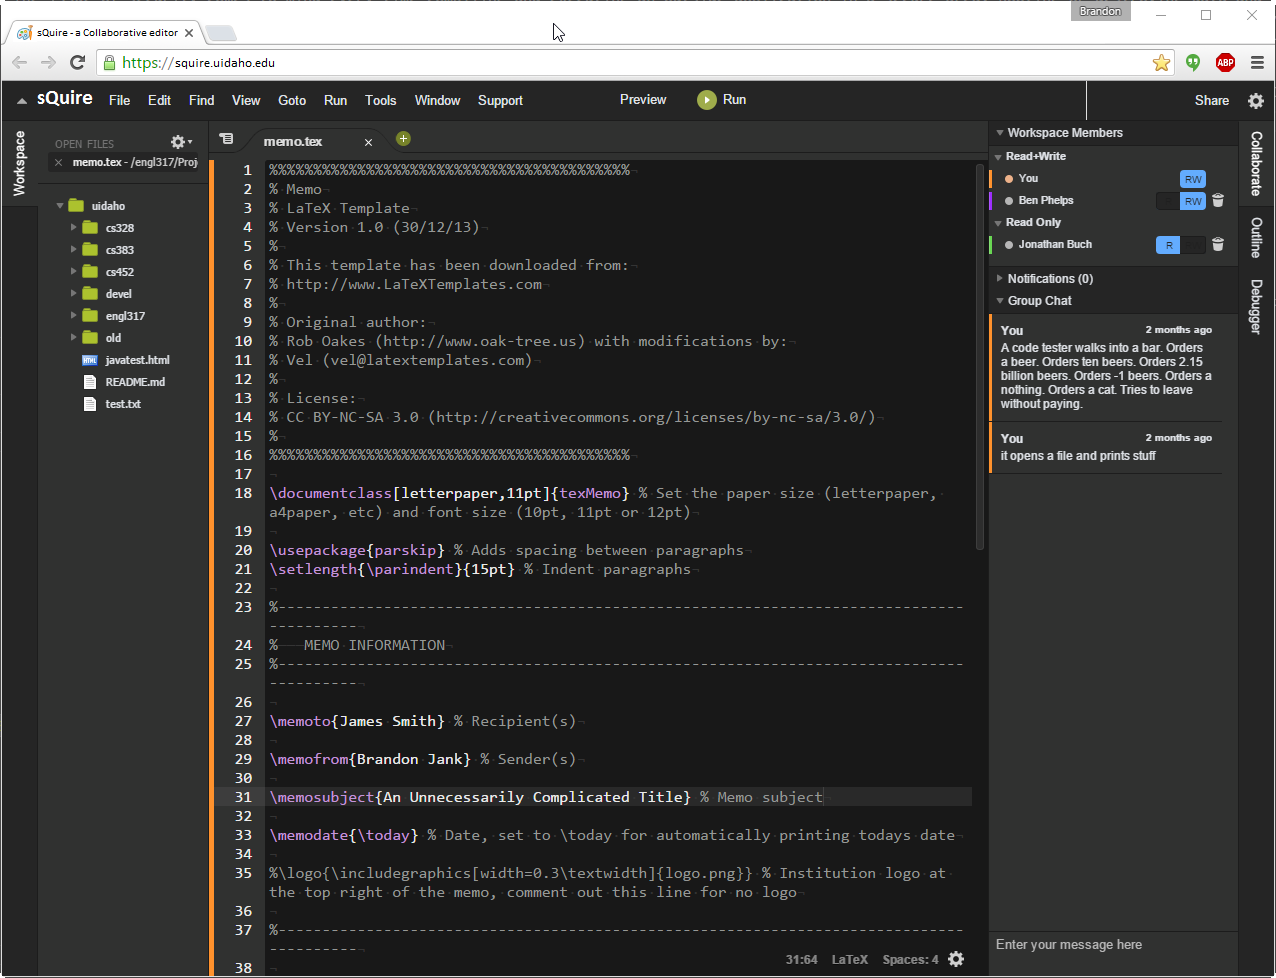
\includegraphics[width=\textwidth]{squire}
    \end{figure}

\section{Use Case Overview (jank6275)}
    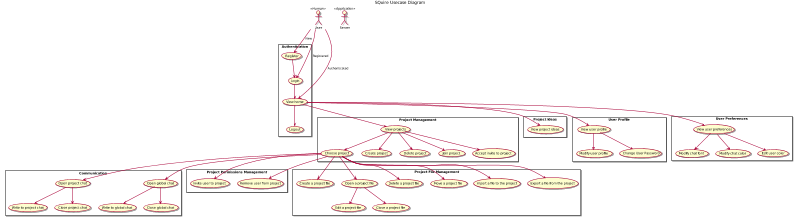
\includegraphics[width=\textwidth]{diagrams/overview-jank6275}
    A usecase diagram that shows all of sQuire\'s features.

\chapter{Requirements Documentation}
    Non-functional requirements describe how the system works, while functional requirements describe what the system should do. Dr. J's list of requirements:
    \begin{itemize}
        \item User profiles should include persistent data including project ownerships and  memberships, friends, e-mail, profile image.
        \item Users should have easy access (background?) awareness information of other users, especially friends and members of shared projects.
        \item Resource defense strategy that includes not subjecting any sQuire server to becoming unresponsive due to a runaway program, and not allowing any sQuire server to give up shell access via an executing program in sQuire.
        \item Indication of who coded what could be background color, underline color, sidebar color, shade/fill pattern, or icon/avatar. 
        \item Since multiple people might edit a given line over its history, support for past history or anyhow multiple persons in this indication is strongly recommended.
        \item Teams should decide whether write access to shared editing should be turn-based or simultaneous
        \item Teams should decide if voice or video is essential. Voice, if supported, might be restricted as to number of listeners and/or number of simultaneous transmitters. Video, if supported, might be restricted as to number of viewers and/or number of simultaneous
        \item Capable of supporting editing, compilation, and execution of Java programs. Programs to be composed as projects and support multiple source code files across multiple directories within a shared top-level directory.
        \item Ability to import/export AND/OR function on projects/source code stored in the ordinary local file system.
        \item Multiuser, up to 32 users can share an IDE session.
        \item Syntax coloring; visual indication to see who coded what.
        \item Shared sessions should allow people to move around their view (read-only, at least) independently, and to quickly jump to where other users are looking.
        \item Users can text chat to individuals, transient shared session members, persistent project member lists, and all logged in users.
    \end{itemize}

\section{Functional Requirements}
    Functional requirements will specify a behaviour or function, for example ``Display the name, total size, available space and format of a flash drive connected to the USB port'' Other examples are ``add customer'' and ``print invoice''. Some of the more typical functional requirements include:
    \begin{itemize}
        \item Authentication (mars2681)
        \item Project Management (mora5651) \begin{itemize}
            \item Admin controls features.  
            \item Public and private sharing of project.
            \item Controlled reading and writing permissions to users. 
            \item Password controls. 
            \item File management. 
            \end{itemize}
        \item Project Ideas (snev7821) \begin{itemize}
            \item Forum to browse potential projects
            \item Up- and down-votes for project selection
            \item Different ways to sort projects (date, projected team size, votes)
            \item Ability to post a project
            \item Ability to delete a project (but only by project author)
            \item Convert potential project stub into active working project \end{itemize}
        \item User Profile (brec9824) \begin{itemize}
            \item User Preferences
            \item User profiles should include persistent data including project ownerships and  memberships, friends, e-mail, profile image. 
            \end{itemize}
        \item Project File Editor (jank6275) \begin{itemize}
            \item Syntax coloring; visual indication to see who coded what. 
            \item Teams should decide whether write access to shared editing should be turn-based or sim
            \item Indication of who coded what could be background color, underline color, sidebar color, shade/fill pattern, or icon/avatar. 
            %\item Indication of who coded what could be background color, underline color, sidebar color, shade/fill pattern, or icon/avatar. Repeat
            \item Write access to shared editing should be simultaneous
            \item Since multiple people might edit a given line over its history, support for past history or anyhow multiple persons in this indication is strongly recommended.    
            \item Multiuser, up to 32 users can share an IDE session.
            \item Shared sessions should allow people to move around their view (read-only, at least) independently, and to quickly jump to where other users are looking. \end{itemize}
        \item Communication (bolt1003) \begin{itemize}
            \item Built-in, global text chat per project.
            \item Private communications between other users.
            \item A friends list with friend status icons and avatar.
            \item A global list of current memembers in the project.
            \item A list of current users working on the project.
            \item A dialog with the user's name and file history when hovering over their icon.
            \item Text chat will be built using standard protocols such as XMPP or IRC.
            \item Allows the use of third-party chat clients.
            \end{itemize}
        \item Security (gall7417) 
        Resource defense strategy that includes not subjecting any sQuire server to becoming unresponsive due to a runaway program, and not allowing any sQuire server to give up shell access via an executing program in sQuire. \begin{itemize}
            \item Require authentication to access all user files and user information.
            \item Ensure confidentiality of all user information.
            \item Use password hashing on a trusted system to ensure password privacy.
            \item Hide password entry on user interface.
            \item Allow password change and reset in case of compromise.
            \item Mitigate security threats by testing against common abuse cases and vulnerabilities.
            \item Validate user integrity before any processing is performed.
            \item Ensure proper character sets for all input given.
            \item All validation failures must result in rejection.
            \item Implement a force halt procedure for runaway programs.
            \item Establish system inactivity timeout after arbitrary amount of time.
            \item Enforce authorization controls on all system requests.
            \item Restrict access to resources and files outside of the users given resources.
            \item Deny access to security protocols and configurations.\end{itemize}
        \item Compiler (boss2849) \begin{itemize}
            \item Capable of supporting editing, compilation, and execution of Java programs. Programs to be composed as projects and support multiple source code files across multiple directories within a shared top-level directory.
            \item Design as a 'plugin' to the system - initial will be a Java compiler, but allow new compiler plugins to be written for other languages.
            \item Compile code for execution within IDE.
            \item Compile code and package to a JAR.
            \item Compile file, file and dependents, project sub-modules, or entire project.
            \item Smart compilation - recompile only what has been changed. 
            \item Allow temporary code freeze before compilation.
            \item Cache snapshots of code on compilation. 
            \end{itemize}
    \end{itemize}
    
\section{Non-Functional Requirements}
    Non-functional requirements cover all the remaining requirements which are not covered by the functional requirements. They specify criteria that judge the operation of a system, rather than specific behaviours, for example: ``Modified data in a database should be updated for all users accessing it within 2 seconds.'' Some typical non-functional requirements are:
    \begin{itemize}
        \item Performance – for example Response Time, Throughput, Utilization, Static Volumetric
        \item Scalability is important to keep in mind during development. The system should be designed in such a way that will easily and reliably scale to accommodate a growing user base. One method of dealing with scalability would be allowing the core system to reactively spawn new slaves to aid in computational needs, such as compilation (as that will be more resource intensive the user base grows). (boss2849)
        \item Capacity (boss2849) \begin{itemize}
            \item Limited space for projects that haven't been initiated (enough for documentation, images, etc.)
            \item Reactively increasing capacity for projects proportional to the absolute needs of the projects. (no fluff)
            \item Encourage developers to store large files elsewhere, e.g. GitHub LFS, AWS, etc.
        \end{itemize}
        \item Availability (brec9824) \begin{itemize}
            \item Since sQuire is web based, downtime for the servers most be kept to a minimum and be no more then once or twice a week for a few hours.
            \item sQuire must be accessible on most browsers 
        \item Reliability (bolt1003) \begin{itemize}
            \item sQuire will be a web application and will leverage the strengths of web technologies to make it reliable.       sQuire will use a webhost such as, Amazon Web services. The webhost's infrastructure provides,                 redunancy for hardware, power and internet service.
        \end{itemize}
        \item Recoverability (mora5651) \begin{itemize}
            \item SQuire will have the ability for the user to save on sQuire's database for recoverability isurance. It will also incorporate autosave feature. 
            \end{itemize}
        \item Maintainability (mora5651) \begin{itemize}
            \item Since sQuire is a web based application running on a webhost. There are 
            many maintenance tools that can be used to track performance. Maintainability of sQuire will also include regular backup schedules, speed test, and security monotoring. 
            \end{itemize}
        \item Serviceability (bolt1003) \begin{itemize}
            \item Running sQuire as a web application allows it to quickly and easily rollback to a previous version or rollforward to a new version. This allows for rapid bug fixing. Infrastructure is redunane so equipment can be taken offline for repair without interupting the users.
        \end{itemize}
        \item Security (jank6275)
        \item Regulatory (mars2681) \begin{itemize}
            \item User upon creating an account must confirm they at least 18 years of age. This is an requirement of COPPA. User must also agree \end{itemize}
        \item Manageability (brec9824) \begin{itemize}
            \item 
        \item Environmental (gall7417) \begin{itemize}
            \item sQuire will run as a browser application in google chrome.
            \item sQire will run on virtually all modern processors.\end{itemize}
        \item Data Integrity (gall7417) \begin{itemize}
            \item sQuire will use tcp to for reliable data communications.
            \item sQuire will use error checking upon large changes to ensure no drastic data corruption occurs.
            \item sQuire will use a history/autosave feature in case of data loss.\end{itemize}
        \item Usability (snev7821) \begin{itemize}
            \item Provides code compilation and file system for users with limited resources. 
            \item Easy to learn system, helpful syntax highlighting.
            \item More satisfying than competitors products, because of social/kickstarter aspect. \end{itemize}
        \item Interoperability (snev7821) \begin{itemize}
            \item Provides github integration
            \item Runs on any of the main browsers (chrome, firefox, IE, safari)
            \item Due to web based design, works on lower end machines \end{itemize}
    \end{itemize}

\section{Unused Requirements}
    \begin{itemize}
        \item Since multiple people might edit a given line over its history, support for past history or anyhow multiple persons in this indication is strongly recommended.
        \item Teams should decide if voice or video is essential. Voice, if supported, might be restricted as to number of listeners and/or number of simultaneous transmitters. Video, if supported, might be restricted as to number of viewers and/or number of simultaneous. - NO, we have skype for a reason.
    \end{itemize}
    
\end{document}